% Figure 1
\begin{figure*}[t]
\centering
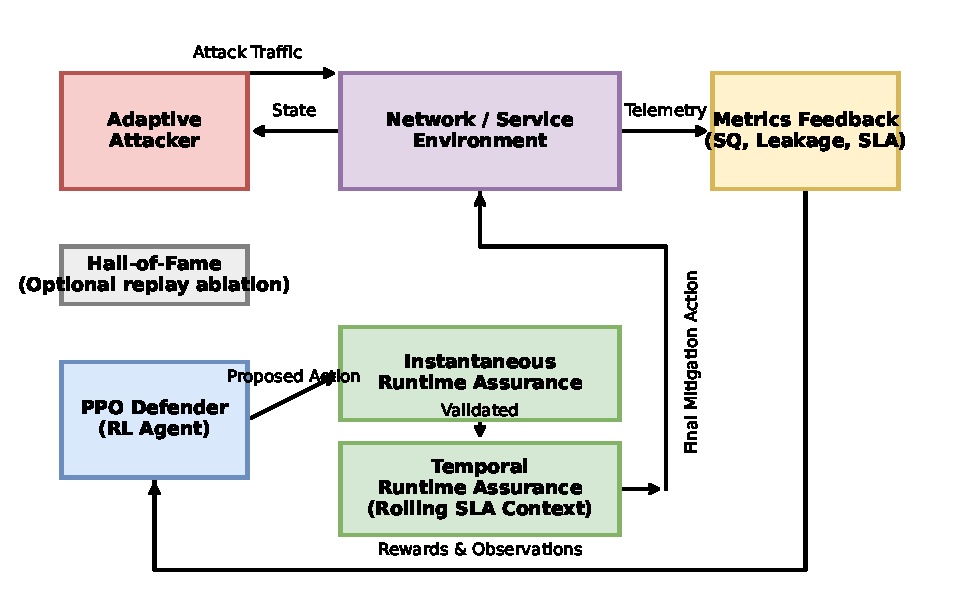
\includegraphics[width=\textwidth]{figures/fig1_architecture.pdf}
\caption{System Architecture. The environment simulates an adaptive attacker targeting a network service. The defender uses PPO to propose mitigation actions, which are evaluated by an Instantaneous Runtime Assurance shield and a Temporal Runtime Assurance shield using rolling/cumulative SLA context. An optional Hall-of-Fame replay ablation evaluates the effect of historical retention on defender plasticity.}
\label{fig:architecture}
\end{figure*}

% Figure 2
\begin{figure*}[t]
\centering
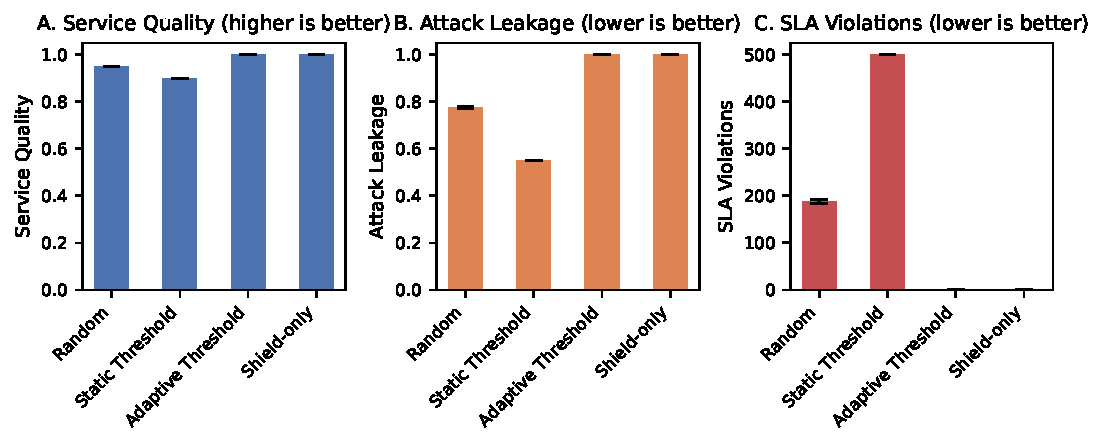
\includegraphics[width=\textwidth]{figures/fig2_baseline_comparison.pdf}
\caption{Baseline defender comparison. The heuristic baselines reveal complementary failure modes: service-preserving policies such as Adaptive Threshold and Shield-only maintain high service quality but allow high attack leakage, whereas more aggressive thresholding reduces leakage at the cost of increased SLA violations. These results motivate learned mitigation with explicit runtime assurance. Higher service quality is better. Lower attack leakage and fewer SLA violations are better.}
\label{fig:baseline_comparison}
\end{figure*}

% Figure 3
\begin{figure*}[t]
\centering
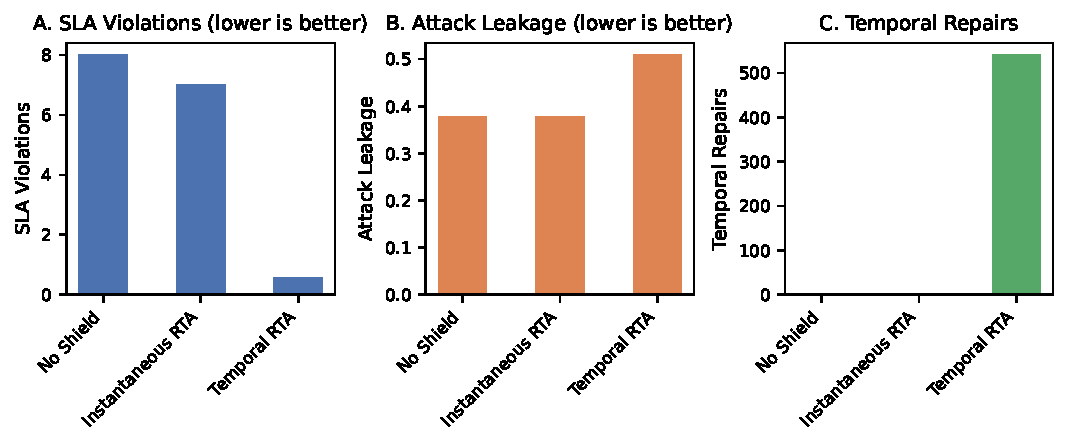
\includegraphics[width=\textwidth]{figures/fig3_temporal_stress_summary.pdf}
\caption{Temporal Runtime Assurance stress validation. Compared with no shielding and instantaneous runtime assurance, Temporal RTA reduced cumulative SLA violations in the evaluated stress setting by using rolling safety context to tighten the admissible action bound. This safety improvement increased attack leakage, illustrating the safety--mitigation trade-off in the modeled simulator. Lower SLA violations and lower attack leakage are better.}
\label{fig:temporal_stress}
\end{figure*}

% Figure 5
\begin{figure}[t]
\centering
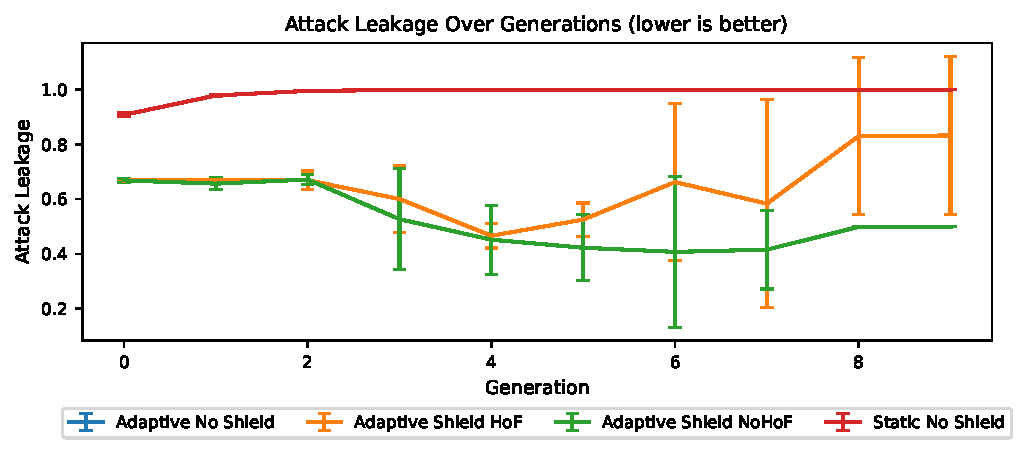
\includegraphics[width=\linewidth]{figures/fig5_adaptive_leakage_generations.pdf}
\caption{Adaptive attacker leakage over generations in the limited-seed co-evolution benchmark. Reactive co-evolution with Temporal RTA and no Hall-of-Fame replay achieved lower leakage than the HoF variant in this configuration. Because this benchmark uses 10 generations and 3 seeds, the trend should be interpreted as limited-seed evidence. Lower attack leakage is better.}
\label{fig:coevolution_trends}
\end{figure}

% Figure 5b
\begin{figure}[t]
\centering
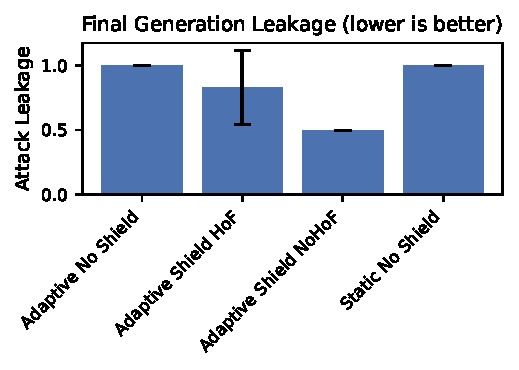
\includegraphics[width=\linewidth]{figures/fig5b_final_generation_leakage.pdf}
\caption{Final generation attack leakage. The bar chart isolates the final generation performance, highlighting the specific leakage bounds achieved by each policy configuration.}
\label{fig:final_generation_leakage}
\end{figure}

% Figure 6
\begin{figure}[t]
\centering
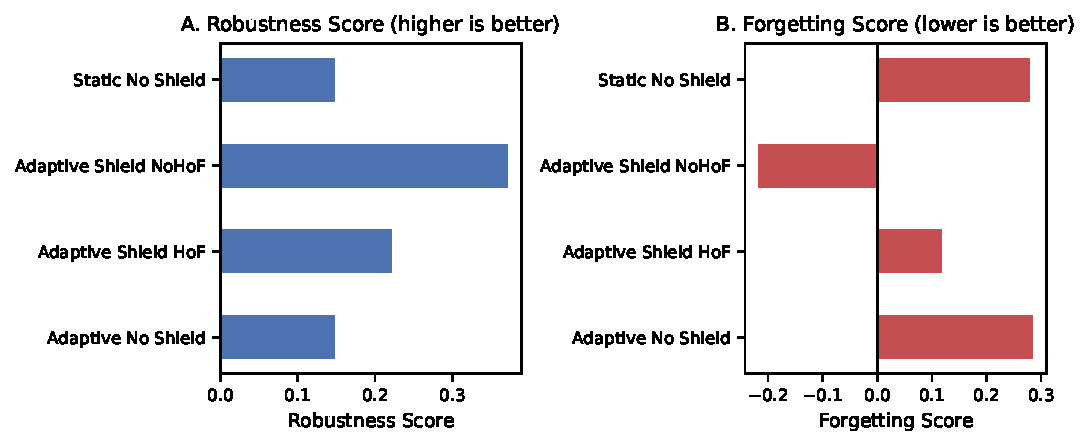
\includegraphics[width=\linewidth]{figures/fig6_hof_ablation.pdf}
\caption{Hall-of-Fame replay ablation. In the limited-seed benchmark, naive HoF replay reduced the multi-objective robustness score and produced a positive forgetting score relative to reactive co-evolution without HoF. This indicates optimization interference from historical replay in the tested configuration. Higher robustness is better. Forgetting score is positive when retention worsens and negative when retention improves.}
\label{fig:hof_ablation}
\end{figure}

% Figure 7
\begin{figure}[t]
\centering
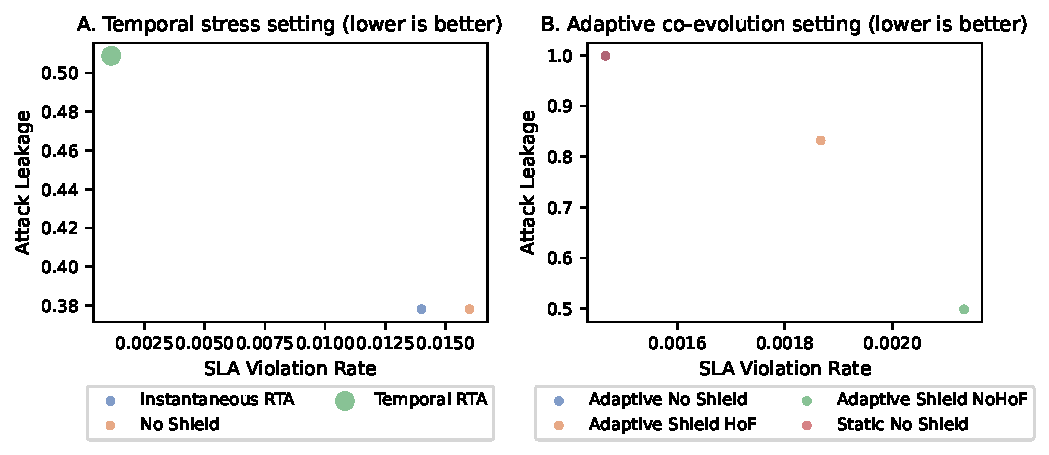
\includegraphics[width=\linewidth]{figures/fig7_safety_performance_tradeoff.pdf}
\caption{Safety--performance trade-off. The temporal stress and adaptive co-evolution results show that reducing SLA-violation risk can increase attack leakage. Marker size indicates shield repair activity. Results are simulator-specific and should be interpreted as evidence of the trade-off. Lower SLA violation rate and lower attack leakage are better.}
\label{fig:tradeoff}
\end{figure}
